\section{Analytische Geometrie}
  \subsection{Dreidimensionaler Raum}
  \begin{definition}
    Der dreidimensionale Raum ist durch $\R^3 = \R \times \R \times \R = \lbrace p_1, p_2, p_3: p_1, p_2, p_3 \in \R \rbrace$. Jeder Punkt $p\in \R^3$ ist eindeutig durch die Angabe seiner Koordinaten $p_1, p_2, p_3)$ bestimmt.
  \end{definition}
  \subsubsection{Abstand}
  \formTab{Euklidischer Abstand zweier Punkte}{d(P,Q)=\sqrt{(p_1-q_1)^2 + (p_2-q_2)^2 + (p_3 - q_3)^2}} 
  \subsubsection{Vektoren} 
  \formTab{Norm eines Vektors}{||x||_{\R^3} = \sqrt{x_1^2 + x_2^2 + x_3^2}}
  Vektoren können skalar multipliziert oder miteinander addiert werden:
  \begin{align}
    \lambda \vecT{x_1 \\ x_2 \\ x_3} &= \vecT{\lambda x_1 \\ \lambda x_2 \\ \lambda x_3}\\
    \vecT{x_1 \\ x_2 \\ x_3} + \vecT{y_1 \\ y_2 \\ y_3} &= \vecT{x_1 + y_1 \\ x_2 + y_2 \\ x_3 + y_3}
  \end{align}   
  \begin{definition}
    Die Koordinaten $P = (p_1, p_2, p_3)$ eines Punktes $p$ definieren den Ortsvektor $p$. Sind zwei Punkte $P,Q$ mit Ortsvektoren $p,q$ gegeben, so gilt 
    \begin{equation}
      d(P,Q) = ||p-q||
    \end{equation}   
  \end{definition}  
    
  \subsubsection{Skalarprodukt}
  Das Skalarprodukt projeziert einen Vektor $b$ auf einen Vektor $a$. Es ist im $\R^3$ definiert als:
  \begin{align}
    (a,b) = <a,b> &= a_1 b_1 + a_2 b_2 + a_3 b_3 \\
    &bzw. \nonumber \\
    (a,b) &= ||a|| \; ||b|| cos \phi
  \end{align}
  Weiterhin gilt:
  \begin{equation}
  ||x|| = \sqrt{x_1^2 + x_2^2 + x_3^2} = \left(\left<\vecT{x_1 \\ x_2 \\ x_3},\vecT{x_1 \\ x_2 \\ x_3}\right>\right)^{\frac{1}{2}} = (x,x)^{\frac{1}{2}}
  \end{equation}
  \begin{definition}
	  $a$ und $b$ heißen orthogonal, falls 
	  \begin{equation*}
	    (a,b) = 0 
	  \end{equation*}
  \end{definition}
  
  \subsubsection{Vektor- bzw. Kreuzprodukt}
  \begin{definition}
    Der Betrag des Vektorproduktes $a\times b$ ist gleich dem Flächeninhalt des von $a$ und $b$ aufgespannten Parallelogramms. Dies folgt direkt aus der Trigonometrie des Dreiecks.
    \begin{equation}
      A = ||a \times b||
    \end{equation}
    Es gilt:
    \begin{equation}
      ||a \times b|| = ||a|| \; ||b|| sin\phi
    \end{equation}    
    Das Vektorprodukt $a \times b$ steht senkrecht auf $a$ und $b$. Die Vektoren $a,b,a \times b$ bilden ein Rechtssystem. $a$: Daumen, $b$: Zeigefinger, $a \times b$: Mittelfinger der rechten Hand.
  Es gelten folgende Eigenschaften:
  \begin{itemize}
    \item[i)   ] $a \times a = 0$
    \item[ii)  ] $a \times b = -b \times a$
    \item[iii) ] $(\lambda a) \times b = \lambda (a \times b)$
    \item[iv)  ] $a \times (b+c) = a \times b + a \times c$
    \item[v)   ]
    \begin{align*}
      \text{Seien }e_1, e_2, e_3\text{ die Einheitsvektoren (siehe HM2) dann gilt:}\\
      e_1 \times e_2 = e_3, \quad e_2 \times e_3 = e_1, \quad e_3 \times e_1 = e_2
    \end{align*}
    \item[vi)   ]
    \begin{equation}
      a := \vecT{a_1 \\ a_2 \\ a_3},\; b := \vecT{b_1 \\ b_2 \\ b_3} \Rightarrow a \times b =  \vecT{a_2 b_3 - a_3 b_2 \\ a_3 b_1 - a_1 b_3 \\ a_1 b_2 - a_2 b_1} 
    \end{equation}
  \end{itemize}
  \end{definition}
  Es gilt die Cauchy-Schwarzsche Ungleichung:
  \begin{align}
    x,y \in \R^n_{\backslash \lbrace 0 \rbrace} &\nonumber \\
    |x \cdot y| &\leq ||x|| \; ||y|| \nonumber \\
    |x \cdot y| &= ||x|| \; ||y|| \Leftrightarrow x = \lambda y \quad, \lambda \in \R
  \end{align}
  
  \subsubsection{Spatprodukt}
  \begin{definition}
    Drei Vektoren $a,b,c$ spannen ein Volumen auf.
    \begin{equation}
      [a,b,c] = (a \times b, c)
    \end{equation}
  \end{definition}
  
  \subsection{Geraden im $\R^2$}
	  \subsubsection{Parameterdarstellung}
	  Die Parameterdarstellung einer Gerade im $\R^2$ ist gegeben mit:
	  \begin{align}
	    x &= a + \lambda(b-a)\quad, \lambda \in \R \nonumber \\
	    &\Rightarrow x = a + \lambda u
	  \end{align}
	  Wobei $u$ die Richtung der Gerade angibt und Richtungsvektor heißt. $a$ heißt Stützvektor.
	  \begin{figure}[htbp] 
		  \centering
		  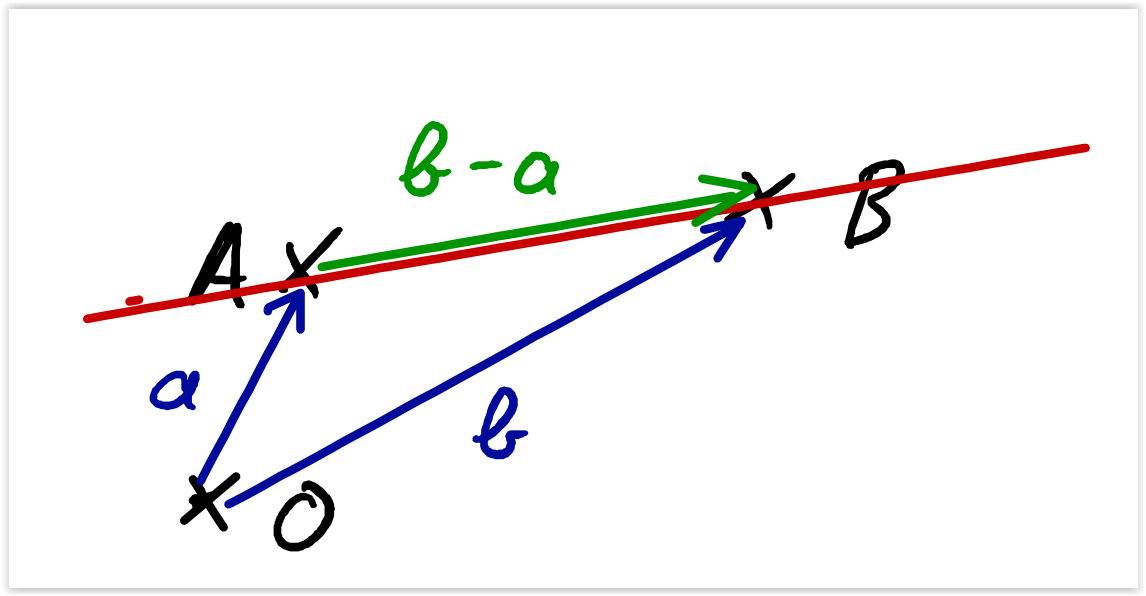
\includegraphics[width=0.7\textwidth]{./img/Geraden.png}
		  \caption{Gerade im $\R^2$\protect\cite{HM12}}
		  \label{fig:gerade_R2}
	  \end{figure}

    \subsubsection{Darstellung in Gleichungs- bzw. Normalform}
    Zur Darstellung in der Normalform muss zunächst ein Normalenvektor $n$ der orthogonal auf $u$ steht gewählt werden, d.h. es muss gelten $(n,u) = 0$.
    \begin{align}
      (n,x) = (n,a + \lambda u) = (n,a) + \lambda \underbrace{(n,u)}_{=0} = (n,a) =: p
    \end{align}
    Die Gleichungsdarstellung ist dann:
    \begin{equation}
      (n,x)-p = 0 
    \end{equation}
    \subsubsection{Hessesche Normalform}
    Zur Bildung der Hesseschen Normalform wird der Normalevektor normiert und es muss $p \geq 0)$ gelten. 
    \begin{equation}
      \left(\frac{n}{||n||},x\right)-p = (n^*,x)-p = 0
    \end{equation}
    \subsubsection{Minimaler Abstand}
    Der Punkt mit minimalem Abstand zum Ursprung $x^*$ auf der Gerade ist der Punkt, an dem der Ortsvektor orthogonal auf der Gerade steht. Das einsetzen dieses Punktes in die Hessesche Normalform liefert also den Abstand zum Ursprung mit:
    \begin{equation}
    (n^*,x^*)=||x^*|| = p = Abstand
    \end{equation}
    \subsubsection{Abstand eines Punktes zur Gerade}
    $\tilde{x}$ sei ein beliebiger Punkt, dann ist
    \begin{equation}
      d = (n^*, \tilde{x})-p
    \end{equation}
    Der Abstand des Punktes zur Geraden.
  \subsection{Geraden und Ebenen im $\R^3$}
    \subsubsection{Parameterdarstellung einer Geraden im $\R^3$}
    \begin{align}
      &g: x = a + \lambda u \quad ,bzw. \nonumber \\
      &g: \vecT{x_1 \\ x_2 \\ x_3} = \vecT{a_1 \\ a_2 \\ a_3} + \lambda \vecT{u_1 \\ u_2 \\ u_3}
    \end{align}
    \subsubsection{Koordinatendarstellung einer Geraden im $\R^3$}
    Eine Gerade lässt sich im $\R^3$ auch als Schnittgerade zweier Ebenengleichungen ausdrücken. Ein Beispiel dazu:
    \begin{align*}
      g: &= \vecT{x_1 \\ x_2 \\ x_3} = \vecT{1 \\ 0 \\ 2} + \lambda \vecT{1\\2\\1} \\
      &\Rightarrow
      \begin{array}{l l l}
        x_1 = 1 + \lambda \\
        x_2 = 2\lambda \\
        x_3 = 2 + \lambda
      \end{array}
      \Rightarrow \lambda = \frac{x_2}{2}\\
      &\Rightarrow x_1 = 1 + \frac{x_2}{2},\quad x3 = 2 + \frac{x_2}{2}
    \end{align*}
    \subsubsection{Parameterdarstellung einer Ebene im $\R^3$}
    \begin{align}
      &E: x = a + \lambda u + \mu v \quad ,bzw. \nonumber \\
      &E: \vecT{x_1 \\ x_2 \\ x_3} = \vecT{a_1 \\ a_2 \\ a_3} + \lambda \vecT{u_1 \\ u_2 \\ u_3} + \mu \vecT{v_1 \\ v_2 \\ v_3}
    \end{align}        
    \subsubsection{Gleichungsdarstellung bzw. Hessesche Normalform einer Ebene im $\R^3$}
    \begin{align}
    &(n^*,x) = (n^*,a) + \lambda \underbrace{(n,u)}_{=0} + \mu \underbrace{(n,v)}_{=0} \nonumber \\
    &\Rightarrow (n^*,x) - (n^*,a) = 0 \quad mit \; (n,a) =: p \nonumber \\
    &\Rightarrow (n^*,x) - p = 0
    \end{align}
    $p$ gibt den Abstand der Gerade zum Ursprung an. $n$ muss auf beiden Richtungsvektoren  senkrecht stehen und lässt sich durch
    \begin{equation}
      n = \frac{u \times v}{|| u \times v||}
    \end{equation}
    bestimmen.
  
    \begin{figure}[htbp] 
		  \centering
		  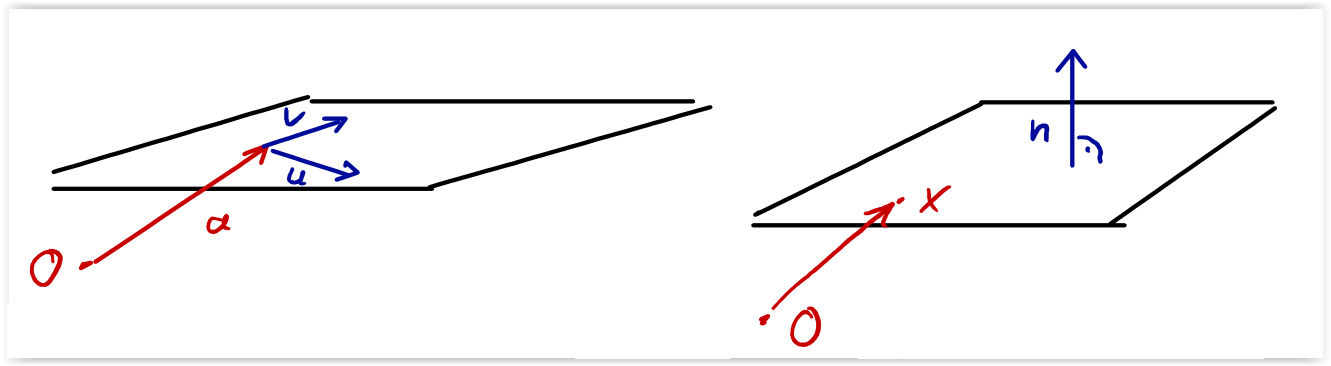
\includegraphics[width=0.7\textwidth]{./img/Ebene_R3.png}
		  \caption{Ebenen im $\R^3$\protect\cite{HM12}}
		  \label{fig:ebene_R3}
	  \end{figure}
	  
	\subsection{Schnitte}
	  \subsubsection{Schnitt zweier Ebenen}
	  Sind die Normalenvektoren nicht parallel existiert eine Schnittgerade. Sie kann durch die entsprechenden Ebenengleichungen beschrieben werden.
	  \begin{align*}
	    E_1 &= \lbrace x\in \R^3:x_1 + 4x_2 = 2 \rbrace \\
	    E_2 &= \lbrace x \in \R^3: x_2 - x_3 = 1\rbrace \\
	    &\Rightarrow n_1 = \vecT{1\\4\\0},\quad n_2 = \vecT{0\\2\\-1} \\ 
	    &\Rightarrow n_1 \; und \; n_2 \;\text{nicht parallel} \Rightarrow \text{Schnittgerade ex.}\\
	    &\Rightarrow g=\lbrace x\in \R^3: x_1 + 4x_2 = 2, x_2 - x_3 = 1\rbrace
	  \end{align*}
	  Der Schnittwinkel zweier Ebenen kann über die jeweiligen Normalenvektoren bestimmt werden.
	  \begin{figure}[htbp] 
		  \centering
		  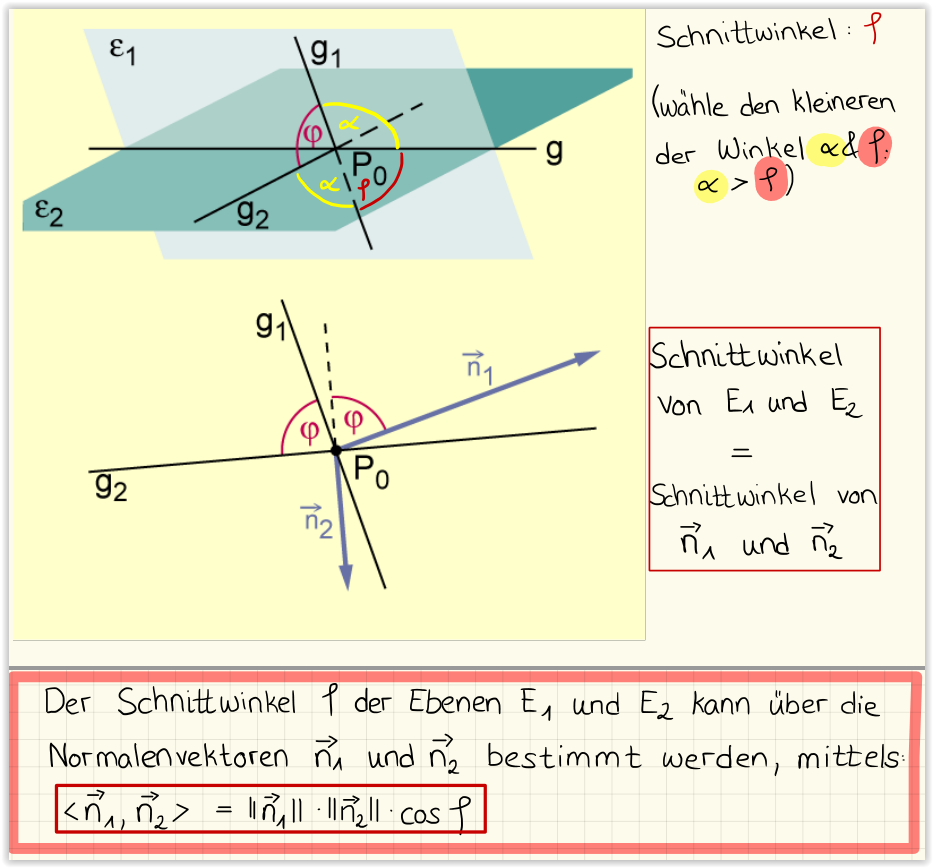
\includegraphics[width=0.67\textwidth]{./img/schnitt_ebene.png}
		  \caption{Schnittwinkel zweier Ebenen\protect\cite{HM1Vortragsubung}}
		  \label{fig:ebene_schnittwinkel}
	  \end{figure} 
	  
	  \subsubsection{Schnitt einer Gerade mit einer Ebene}
	  Dort wo sich Ebene und Gerade schneiden muss der Punkt beide Gleichungen erfüllen. Um dies zu prüfen, setzt man dei Parameterdarstellung der Gerade in die Ebene ein. Erhält man einen Punkt, so ist dies der Punkt an dem sich beide schneiden.
	  \subsubsection{Schnitt zweier Geraden im $\R^3$}
	  Es seien $g_1$ und $g_2$ zwei Geraden mit
	  \begin{align*}
	    g_1: x = a + \lambda u \quad, \lambda \in \R\\
	    g_2: y = b + \mu v \quad, \mu \in \R
	  \end{align*}
	  Es existieren grundsätzlich drei Fälle:
	  \begin{itemize}
	    \item Es existiert ein Schnittpunkt \\
	      Schnittbedingung: $x = y$
	    \item Beide Geraden sind parallel \\
	      Bedingung: $u = \theta v \quad, \theta \in \R$
	    \item Die Geraden schneiden sich nicht und $u$ ist nicht parallel zu $v$ (windschief)
	  \end{itemize}
	  Für windschiefe Geraden ist der minimale Abstand durch die Bedingung $(x-y) \bot u,\; (x-y) \bot v$ gegeben.
	  \subsubsection{Abstand zweier Geraden im $\R^3$}
	  Hierzu stellt man Hilfsebenen auf.
	  \begin{align*}
	    g_1 \Rightarrow E_1: x = a + \lambda u + \mu v \\
	    g_2 \Rightarrow E_2: y = b + \lambda u + \mu v
	  \end{align*}
	  \begin{figure}[H] 
		  \centering
		  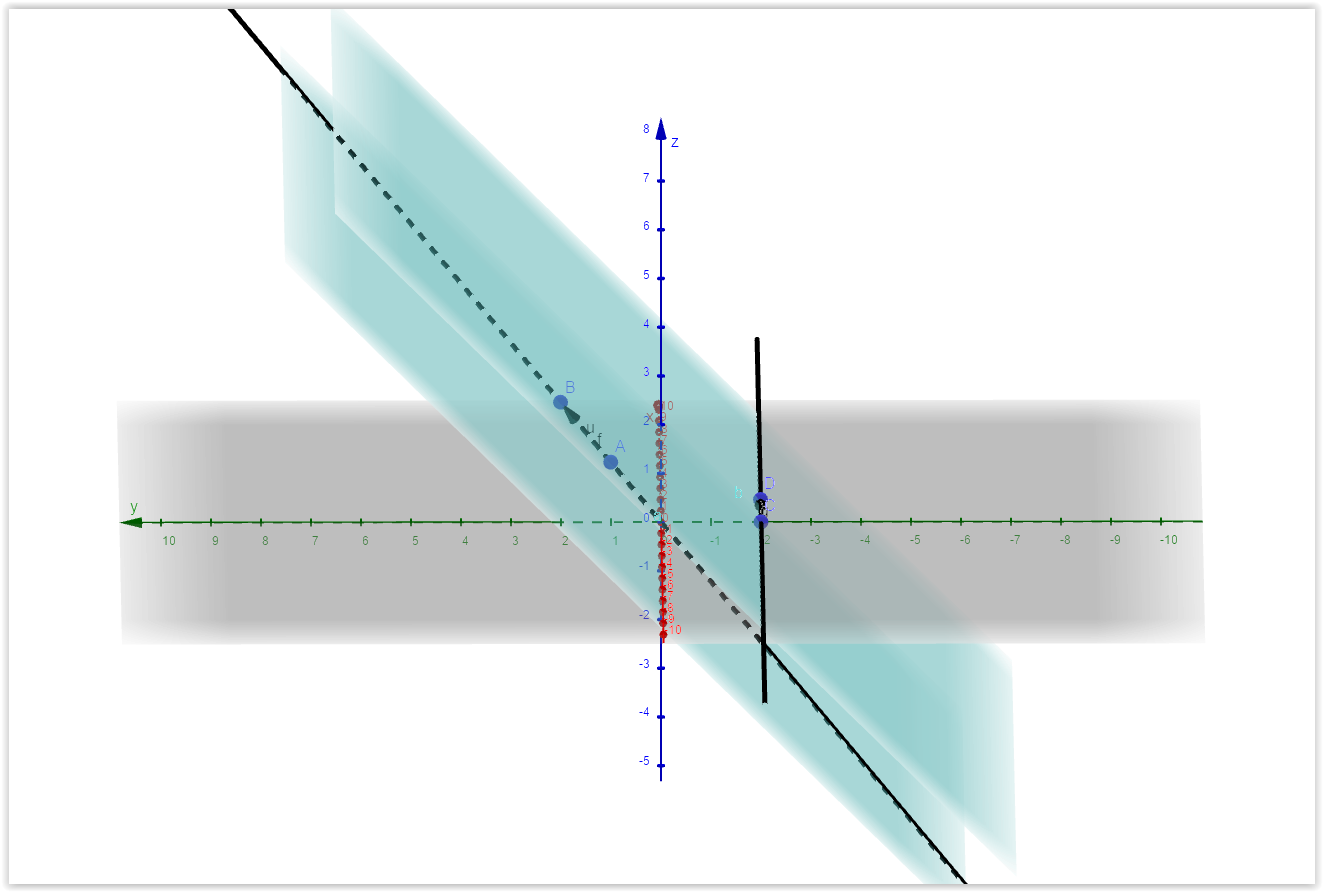
\includegraphics[width=0.5\textwidth]{./img/Abstand_Geraden.png}
		  \caption{Abstand zweier Geraden $\R^3$}
		  \label{fig:abstand_geraden}
	  \end{figure}
	  Zur Bestimmung kann man den Abstandes vom Punkt $a$ (oder jeder andere Punkt auf $g_1$ zur Ebene $E_2$ bestimmen. Hierzu wird die hessesche Normalform von $E_2$ gebildet und $a$ eingesetzt.
\newpage